As detailed in \refsec{sources of helium}, helium can be produced in tungsten from neutron \gls{transmutation} and from tritium decay.
This section will focus on comparing these two indirect sources with direct helium implantation in \glspl{monoblock}.

\subsection{Neutron induced transmutation}

In combination with the \gls{paramak} code \sidecite{shimwell_paramak_2021} used for creating the geometry, a neutronics simulation was run to assess the total quantity of helium generation in a \gls{monoblock} under neutron irradiation with the \gls{openmc} code \sidecite{romano_openmc_2015}, a modern open-source Monte-Carlo neutron and photon transport code.
In this simulation, a neutron source was placed above the \gls{monoblock} and the total helium production was tallied.
The neutron source corresponds to a \SI{500}{MW} DT neutron source, which gives a neutron generation rate of \SI{1.8e20}{neutrons.s^{-1}} (based on the energy produced by the DT fusion reaction).
50 batches of 1 million neutrons were simulated in order to reduce the stochastic error inherant to Monte-Carlo methods.

The production of helium was found to be more important close to the top surface and to the neutron source (see \reffig{transmutation helium in monoblock}).
It evolves as linearly with the distance from the top surface.
The maximum generation rate is $\approx \SI{7e18}{m^{-3}.s^{-1}}$, which is well below the generation rate from direct implantation.
\reffig{helium generation distribution} was obtained by averaging all the values by distance from the top surface.
The error bars were computed by averaging the standard deviation provided by \gls{openmc}.

\begin{figure*}
    \centering
    \begin{subfigure}{0.5\linewidth}
        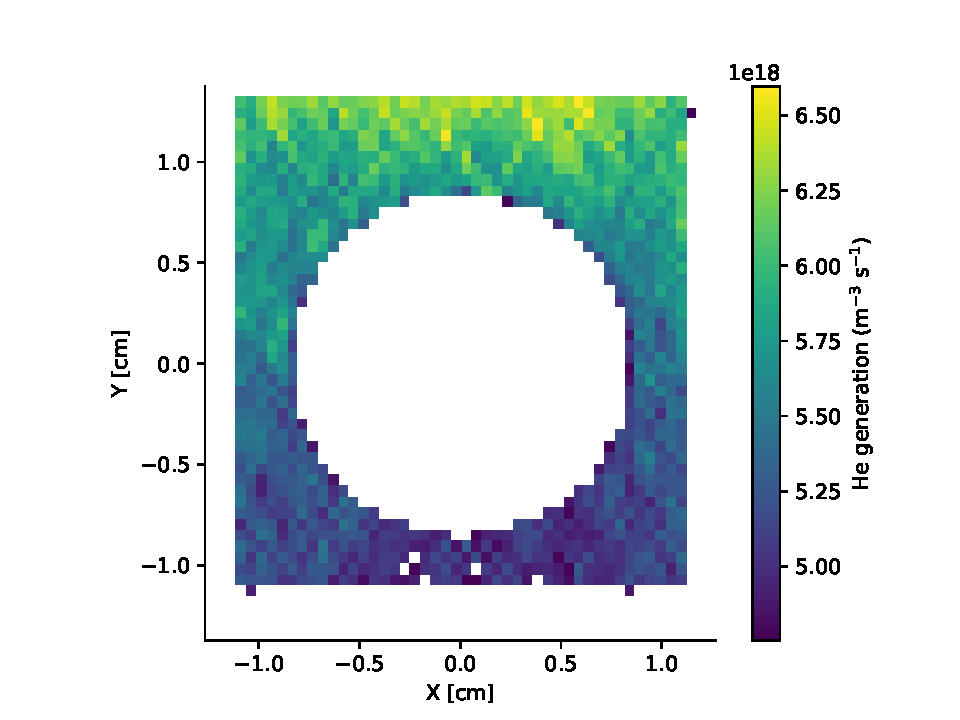
\includegraphics[width=\linewidth]{Figures/Chapter5/helium_transmutation_in_monoblock.pdf}
        \caption{2D distribution.}
    \end{subfigure}%
    \begin{subfigure}{0.5\linewidth}
        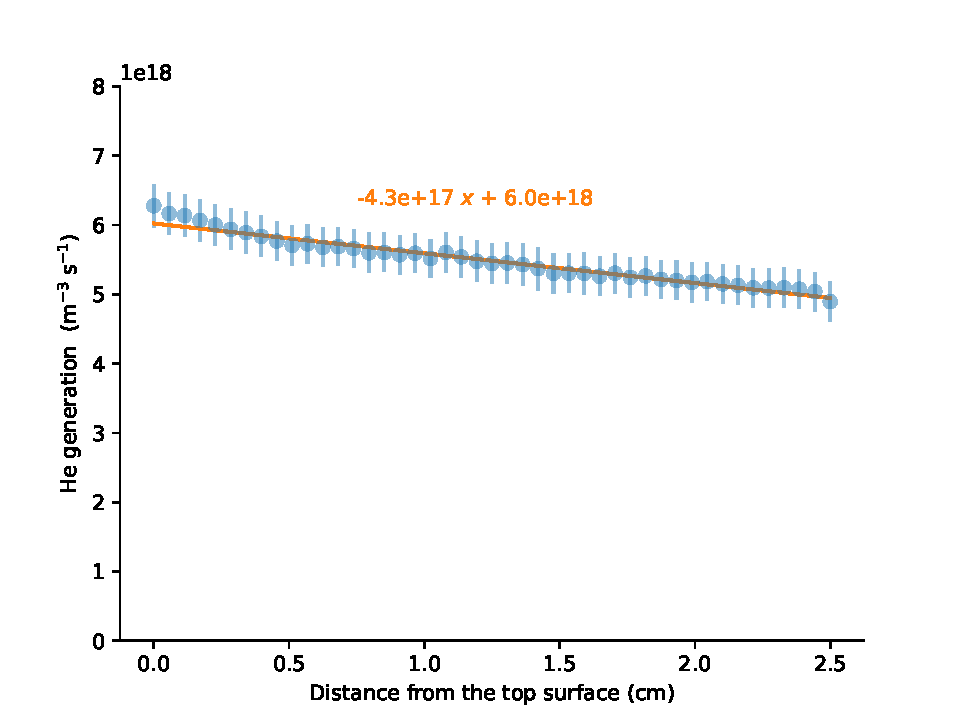
\includegraphics[width=\linewidth]{Figures/Chapter5/he_generation_distribution.pdf}
        \caption{Distribution from the top surface. Errors bars correspond to the 95 \% confidence interval.}
        \labfig{helium generation distribution}
    \end{subfigure}
    \caption{Helium generation via transmutation in a \gls{monoblock} (only tungsten is shown).}
    \labfig{transmutation helium in monoblock}
\end{figure*}

Note that this is a conservative case as the \gls{monoblock} simulated is right below the neutron source.
Other \glspl{monoblock} of the \gls{divertor} will be tilted and shadowed by others and therefore will interact less with the neutrons.


\subsection{Tritium decay}

The generation of helium via tritium decay was computed from \gls{festim} simulations of hydrogen transport in \glspl{monoblock}.
For this case, a volumetric source was added to take the radioactive decay into account.
\refeq{mobile} and \refeq{trapped} can be written as:

\begin{equation}
    \frac{\partial c_\mathrm{m}}{\partial t}=\nabla \cdot (D \nabla c_\mathrm{m} ) -\sum \frac{\partial c_{\mathrm{t}, i}}{\partial t} - \lambda_\mathrm{decay} c_\mathrm{m}
\end{equation}

\begin{equation}
    \frac{\partial c_{\mathrm{t}, i}}{\partial t}=k_i \cdot c_\mathrm{m} \cdot\left(n_{i}-c_{\mathrm{t}, i}\right)-p_i \cdot c_{\mathrm{t}, i} - \lambda_\mathrm{decay} c_{\mathrm{t}, i}
\end{equation}
where $\lambda_\mathrm{decay}$ is the decay constant in \si{s^{-1}}.
The decay constant is expressed from the tritium radioactive half-life $\tau_{1/2}$:
\begin{equation}
    \lambda_\mathrm{decay} = \frac{\ln 2}{\tau_{1/2}} \approx \SI{1.77e-9}{s^{-1}}
\end{equation}

The generation rate of helium from tritium decay is directly proportional to the hydrogen (tritium) retention can therefore be expressed as $\lambda_\mathrm{decay} (c_\mathrm{m} + \sum c_{\mathrm{t}, i})$.
In order to remain conservative, it was computed at steady state.

The maximum generation rate of helium in the \gls{monoblock} was found to be \SI{6.5e12}{m^{-3}.s^{-1}} (see \reffig{he generation from t decay}).
This value assumes all the implanted hydrogen is tritium and should be halved to consider a 50\%-50\% DT mixture.
This is order of magnitudes below the generation from direct implantation.

\begin{figure}
    \centering
    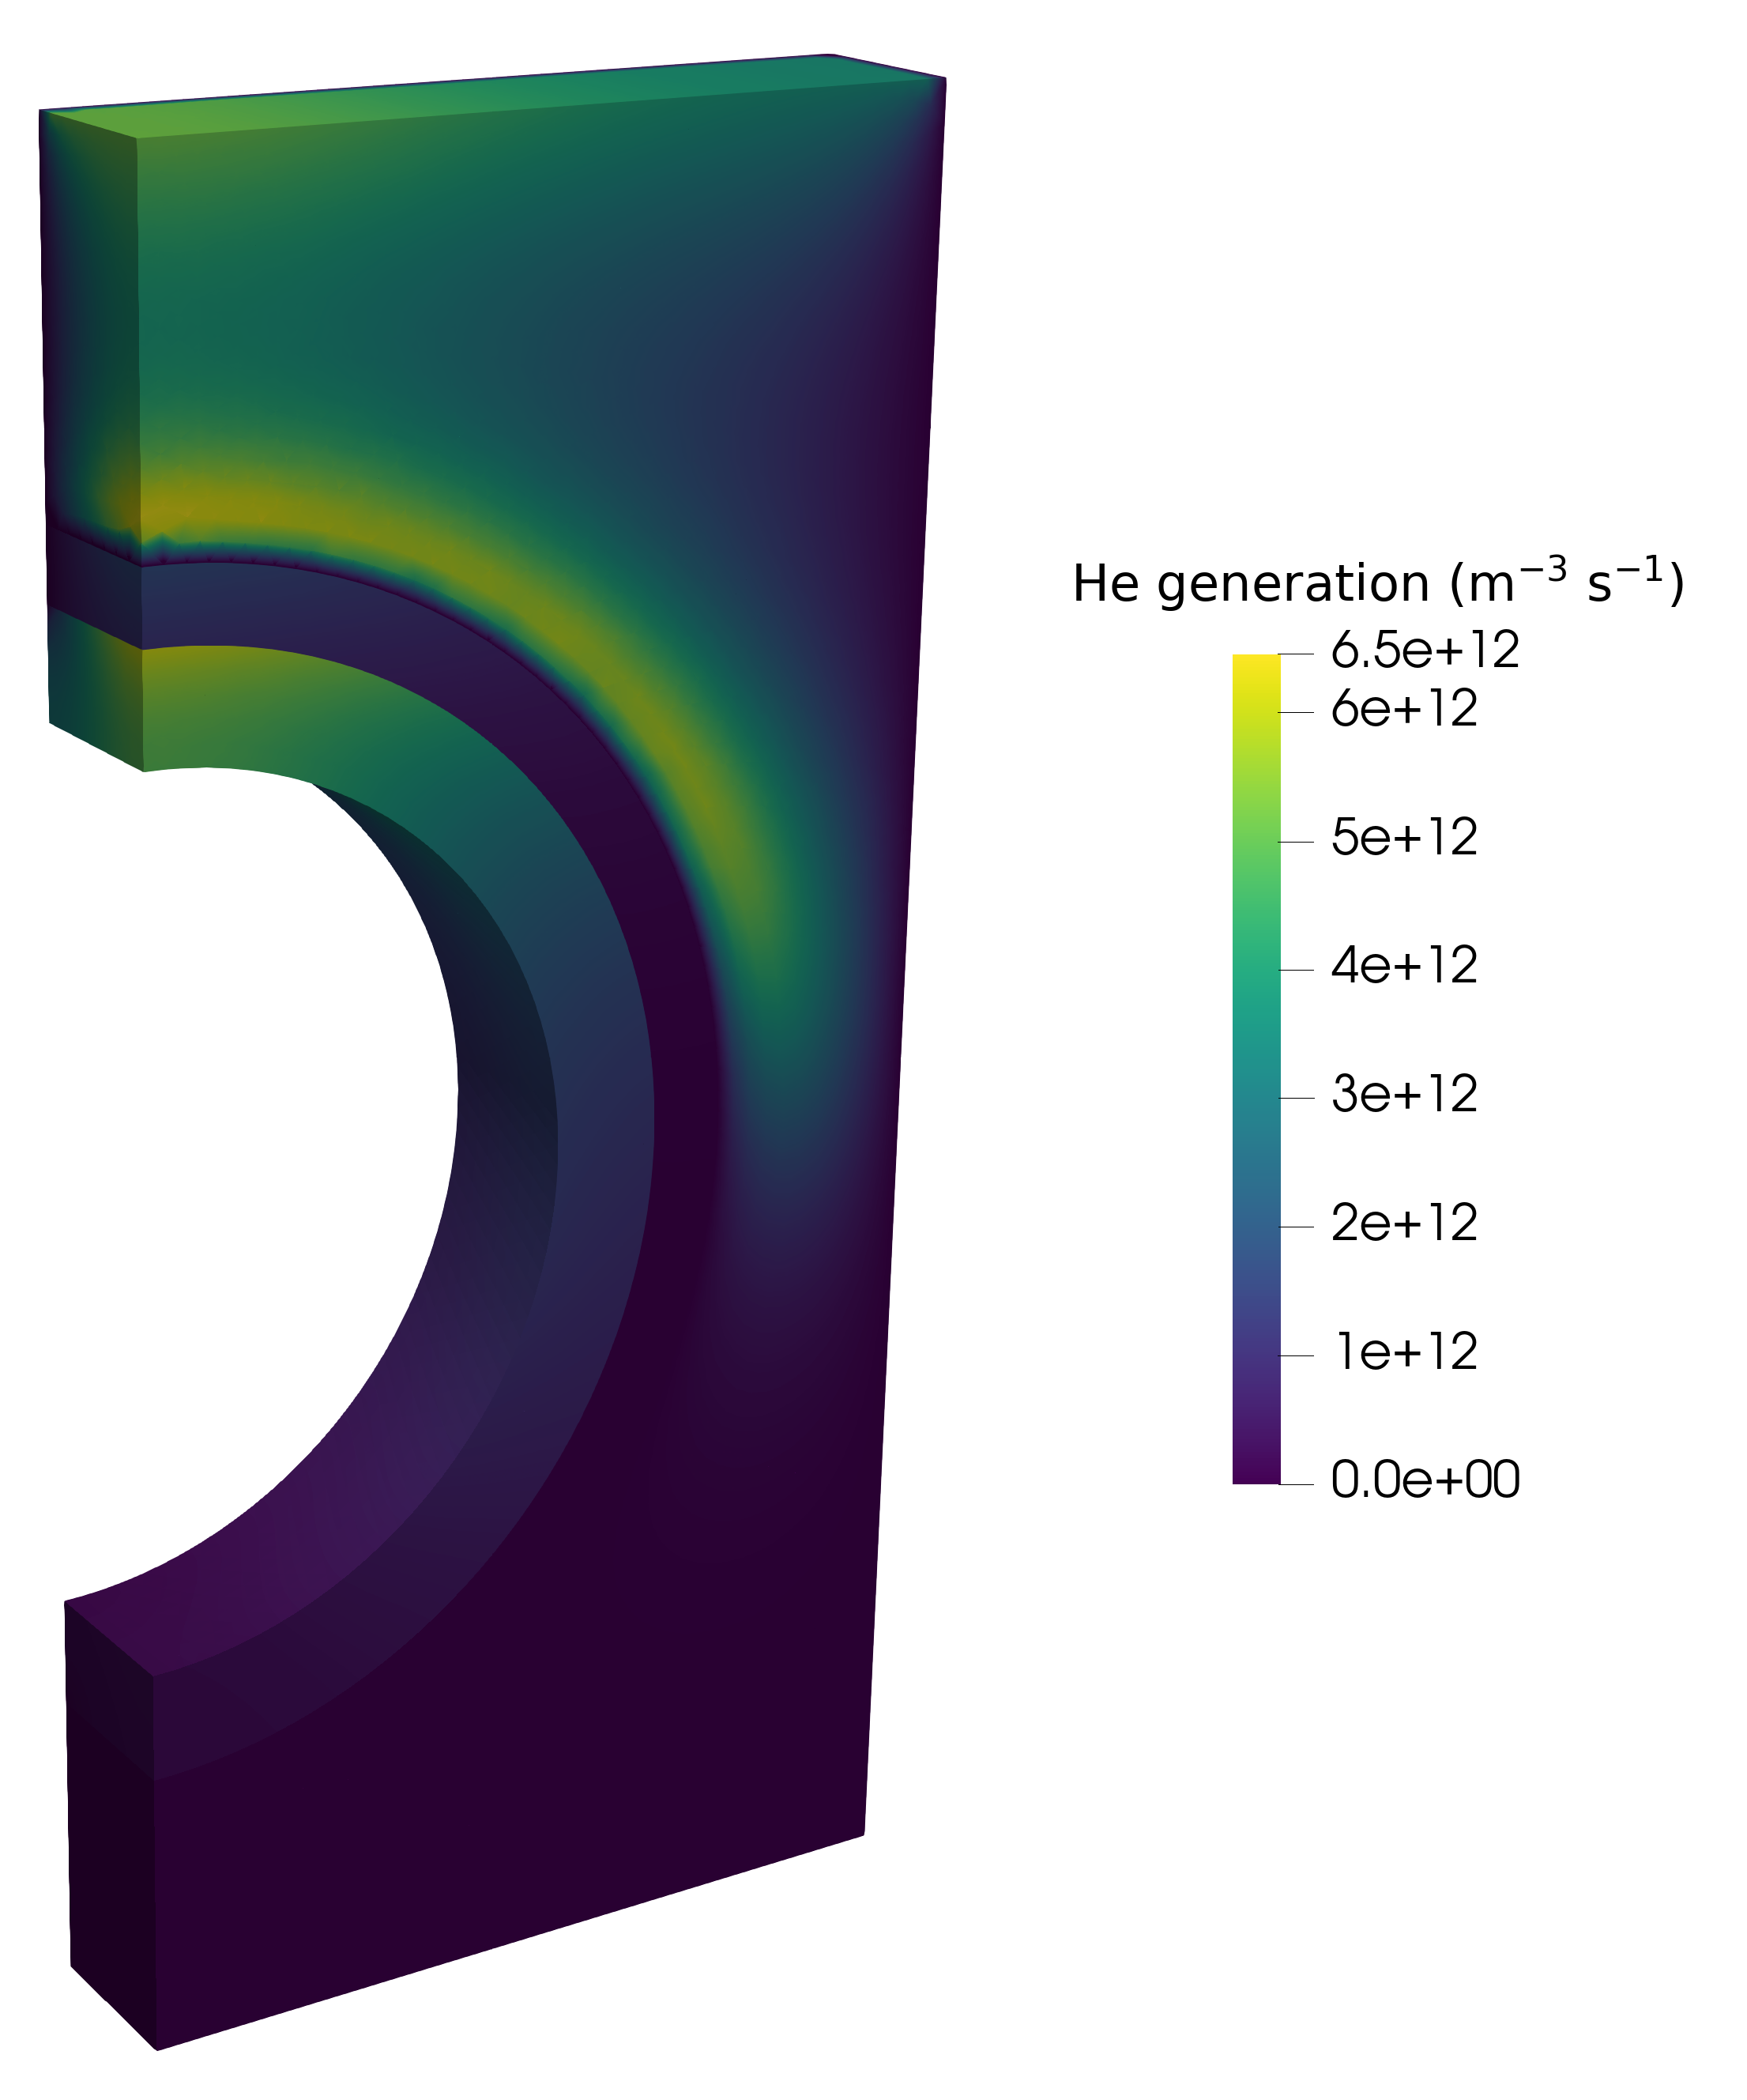
\includegraphics[width=0.5\linewidth]{Figures/Chapter5/he_generation_decay.png}
    \caption{Steady state helium generation from tritium decay in a monoblock.}
    \labfig{he generation from t decay}
\end{figure}


When comparing the production of helium from indirect sources with the quantity helium implanted from the plasma, it appears that the indirect sources are negligible (see \reffig{comparison helium generation}).

\begin{figure}
    \centering
    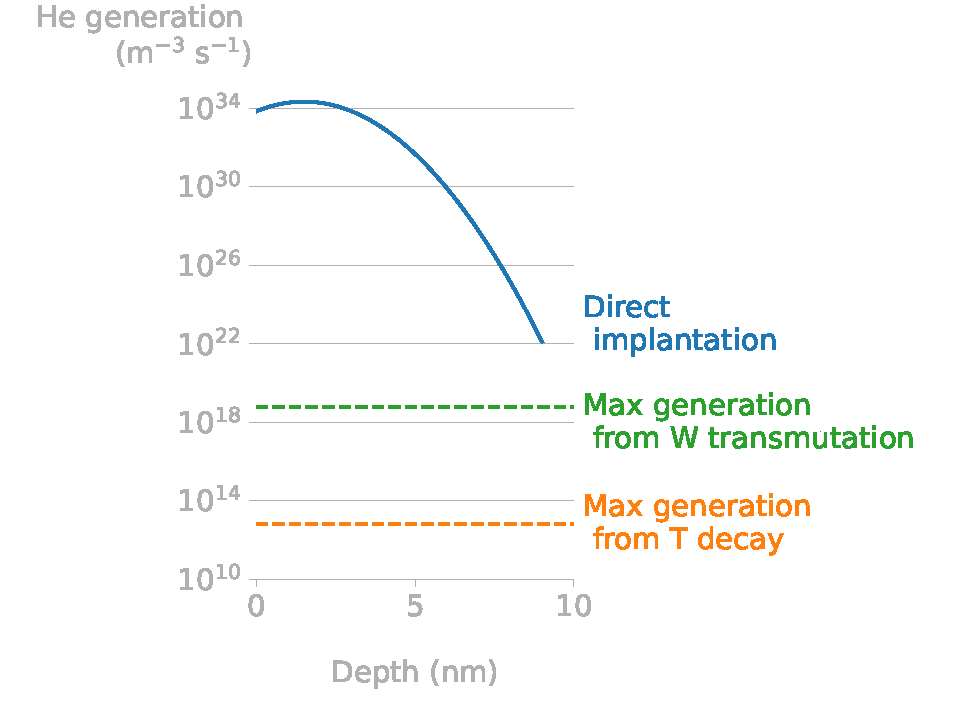
\includegraphics[width=\linewidth]{Figures/Chapter5/helium_generation.pdf}
    \caption{Comparison of the three sources of helium in a \gls{monoblock}. The source from direct implantation was computed for an incident flux of \SI{5e25}{m^{-2}.s^{-1}} with a gaussian distribution (mean of \SI{1}{nm} and standard deviation of \SI{1.5}{nm}).}
    \labfig{comparison helium generation}
\end{figure}